\documentclass[border=12pt]{standalone}
\usepackage{tikz}

\begin{document}
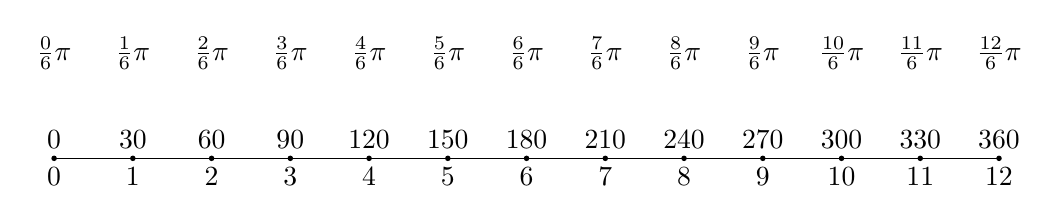
\begin{tikzpicture}
\draw (0,0) -- (12,0);
\foreach \x in {0,...,12} {
		\fill (\x,0) circle(1pt); 
    \node at (\x, 0) [below]{\x}; % 下方显示 \x
}		
\foreach \x [evaluate=\x as \result using int(\x*30)] in {0,...,12} {
    \node at (\x, 0) [above]{\result}; % 上方显示\result
    \node at (\x, 1) [above]{$\frac{\x}{6}\pi$}; % 上方显示\rad  
}
\end{tikzpicture}
\end{document}